\documentclass[12pt,a4paper]{report}

% Packages for layout and styling
\usepackage[utf8]{inputenc}
\usepackage[T1]{fontenc}
\usepackage{geometry}
\geometry{top=1in, bottom=1in, left=1in, right=1in}
\usepackage{graphicx}
\usepackage{amsmath}
\usepackage{amssymb}
\usepackage{hyperref}
\usepackage{booktabs}
\usepackage{caption}
\usepackage{subcaption}
\usepackage{float}
\usepackage{titlesec}
\usepackage{fancyhdr}
\usepackage{array}
\usepackage{longtable}
\usepackage{tikz}
\usetikzlibrary{shapes,arrows,positioning,calc}

% Header and Footer configuration
\pagestyle{fancy}
\fancyhf{}
\fancyhead[L]{\textit{TransGraph-PPI: Hybrid Ensemble Framework for PPI Prediction}}
\fancyfoot[L]{Dept. of CSE, St Joseph Engineering College, Mangaluru -- 2026-27}
\fancyfoot[R]{Page \thepage}
\renewcommand{\headrulewidth}{0.4pt}
\renewcommand{\footrulewidth}{0.4pt}

% Remove "Chapter N" from chapter headings
\titleformat{\chapter}[display]
  {\normalfont\huge\bfseries}{\chaptertitlename\ \thechapter}{20pt}{\Huge}
\titlespacing*{\chapter}{0pt}{-30pt}{20pt}

\begin{document}

% --- Page 1: Title Page ---
\begin{titlepage}
    \begin{center}
        {\Large \textbf{Visvesvaraya Technological University, Belagavi – 590018}} \\[1.5cm]
        
        % Logo (Placeholder for the VTU logo)
        % \includegraphics[width=0.2\textwidth]{vtu_logo.png} \\[1cm]
        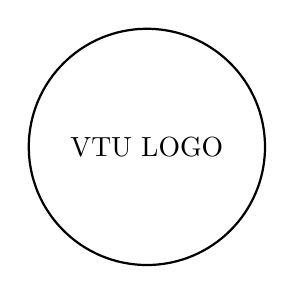
\begin{tikzpicture}
            \draw[thick] (0,0) circle (1.5cm);
            \node at (0,0) {VTU LOGO};
        \end{tikzpicture} \\[1cm]

        {\Large \textbf{LITERATURE SURVEY}} \\[0.5cm]
        {\Large \textbf{ON}} \\[0.5cm]
        {\Large \textbf{TransGraph-PPI: A Hybrid Ensemble Framework for Sequence-Based Protein–Protein Interaction Prediction}} \\[1.5cm]

        \textit{Submitted in partial fulfillment of the requirements for the degree} \\[0.2cm]
        {\large \textbf{BACHELOR OF ENGINEERING}} \\[0.2cm]
        \textit{in} \\[0.2cm]
        {\large \textbf{COMPUTER SCIENCE \& ENGINEERING}} \\[1.5cm]

        \textit{Submitted by} \\[0.5cm]
        \begin{tabular}{ll}
            \textbf{Ajay Preenal Dsouza} & \textbf{4SO23CS008} \\
            \textbf{Ashwini Shenoy B} & \textbf{4SO23CS042} \\
            \textbf{Basil S} & \textbf{4SO23CS050} \\
            \textbf{Bhavish V} & \textbf{4SO23CS052} \\
        \end{tabular} \\[1cm]

        \textit{Under the Guidance of} \\[0.2cm]
        {\large \textbf{Ms Jaishma Kumari B}} \\[0.1cm]
        \textit{Assistant Professor, Department of CSE} \\[1cm]

        % Logo (Placeholder for the College logo)
        % \includegraphics[width=0.25\textwidth]{college_logo.png} \\[1cm]
        
\begin{tikzpicture}
            \draw[thick] (0,0) rectangle (3,2);
            \node at (1.5,1) {COLLEGE LOGO};
        \end{tikzpicture} \\[1cm]

        {\large \textbf{DEPT. OF COMPUTER SCIENCE AND ENGINEERING}} \\[0.2cm]
        {\large \textbf{ST JOSEPH ENGINEERING COLLEGE}} \\[0.1cm]
        \textbf{An Autonomous Institution} \\[0.1cm]
        {\small (Affiliated to VTU Belagavi, Recognized by AICTE)} \\[0.1cm]
        \textbf{Vamanjoor, Mangaluru - 575028, Karnataka} \\[0.5cm]
        \textbf{2026-27}
    \end{center}
\end{titlepage}

\pagenumbering{roman}
\newpage

% --- Page 2: Table of Contents ---
\setcounter{page}{2}
\tableofcontents
\newpage

% --- Page 3: Chapter 1 Introduction ---
\pagenumbering{arabic}
\setcounter{page}{3}
\chapter{Literature Survey}

This chapter presents a comprehensive review of ten recent and significant research papers related to sequence-based Protein–Protein Interaction (PPI) prediction. Each paper is analyzed with respect to the problem identified, methodology, implementation details, results, inferences, and limitations. The review concludes with a comparison table summarizing the key findings across all reviewed works.

\newpage

% --- Page 4: Section 1.1 ---
\section{Sequence-Based Protein–Protein Interaction Prediction and Its Applications in Drug Discovery}
\textbf{Authors:} Fran\c{c}ois Charih, James R. Green, and Kyle K. Biggar \\
\textbf{Published in:} \textit{Cells}, vol. 14, no. 18, p. 1449, Sep. 2025.

\begin{table}[H]
\centering
\renewcommand{\arraystretch}{1.5}
\begin{tabular}{|p{0.25\textwidth}|p{0.7\textwidth}|}
\hline
\textbf{Problem Identified} & Protein–Protein Interactions (PPIs) play a crucial role in biological processes such as signal transduction, immune response, and cellular regulation. Identifying these interactions experimentally using methods such as yeast two-hybrid or mass spectrometry is expensive, time-consuming, and difficult to scale for large protein datasets. There is therefore a need for computational methods that can accurately predict PPIs using only protein sequence data, enabling faster analysis and supporting drug discovery. \\ \hline
\textbf{Methodology} & The paper provides a comprehensive survey of modern computational approaches for sequence-based PPI prediction. It covers traditional machine learning models including Support Vector Machines (SVMs), Random Forests, and Multi-layer Perceptrons (MLPs), as well as deep learning models such as Convolutional Neural Networks (CNNs), Recurrent Neural Networks (RNNs), and transformer-based protein language models. The survey treats PPI prediction as a binary classification problem and evaluates approaches based on their ability to distinguish interacting from non-interacting protein pairs. \\ \hline
\textbf{Implementation Details} & Protein interaction data is drawn from publicly available databases including BioGRID, STRING, IntAct, and MINT. Protein sequences are retrieved from UniProt/Swiss-Prot. Feature extraction techniques surveyed include amino acid composition (AAC), pseudo amino acid composition (PseAAC), conjoint triad features, Position-Specific Scoring Matrix (PSSM), and protein language model embeddings. Models are evaluated on standard metrics: Accuracy, Precision, Recall, F1-Score, ROC-AUC, and Precision-Recall Curve (AUPRC). \\ \hline
\end{tabular}
\end{table}

\newpage

% --- Page 5: Section 1.1 (Continued) ---
\begin{table}[H]
\centering
\renewcommand{\arraystretch}{1.5}
\begin{tabular}{|p{0.25\textwidth}|p{0.7\textwidth}|}
\hline
\textbf{Results} & Deep learning models, particularly those employing transformer-based protein embeddings, achieve substantially improved performance compared to traditional machine learning methods. The survey demonstrates that protein language model embeddings---trained on large-scale protein sequence corpora---capture contextual, evolutionary, and biochemical information that enhances PPI prediction accuracy. \\ \hline
\textbf{Inference / Findings} & The study concludes that sequence-based computational approaches provide a scalable and efficient alternative to experimental PPI detection. Deep learning and protein language models significantly improve prediction accuracy. Sequence-based methods are more broadly applicable than structure-based approaches because protein sequence data is readily available. Accurate PPI prediction can assist in drug target identification and therapeutic design. \\ \hline
\textbf{Limitations / Future Scope} & Challenges remain including class imbalance between interacting and non-interacting protein pairs, dataset bias due to limited experimentally validated interactions, difficulty generalizing models to new species or unseen proteins, and the need for better integration of sequence, structural, and network-level information. Future research should focus on hybrid models combining protein language models, graph neural networks, and ensemble techniques. \\ \hline
\end{tabular}
\end{table}

\newpage

% --- Page 6: Section 1.2 ---
\section{Advances in Protein–Protein Interaction Prediction: A Deep Learning Perspective}
\textbf{Authors:} Noor Alkhateeb and Mamoun Awad \\
\textbf{Published in:} \textit{Bioinformatics Journal Review}, 2023.

\begin{table}[H]
\centering
\renewcommand{\arraystretch}{1.5}
\begin{tabular}{|p{0.25\textwidth}|p{0.7\textwidth}|}
\hline
\textbf{Problem Identified} & Protein–Protein Interactions are fundamental to many biological processes such as signal transduction, metabolic regulation, immune response, and cell cycle control. Experimental techniques for detecting PPIs, including yeast two-hybrid screening and co-immunoprecipitation, are expensive, time-consuming, and prone to false positives or negatives. There is a growing need for computational methods that can efficiently predict PPIs from biological data. Challenges such as complex protein structures, noisy datasets, and severe class imbalance make accurate prediction difficult. \\ \hline
\textbf{Methodology} & The paper provides a comprehensive review of deep learning approaches for PPI prediction, categorizing methods by architecture type. Major architectures discussed include Deep Neural Networks (DNN), Convolutional Neural Networks (CNN), Recurrent Neural Networks (RNN), Graph Convolutional Networks (GCN), and Ensemble Learning Models. The typical workflow involves feature extraction, dimensionality reduction, model training, and interaction probability prediction. \\ \hline
\textbf{Implementation Details} & Datasets used include STRING, UniProt, DIP (Database of Interacting Proteins), HIPPIE, and HPRD. Features include both sequence-based (PSSM, amino acid sequences, evolutionary conservation, ProtVec embeddings) and physicochemical features (hydrophobicity, polarizability, side-chain volume, electrostatic properties). Performance is evaluated using Accuracy, Precision, Recall, F1-score, and ROC-AUC. \\ \hline
\textbf{Results} & Deep learning approaches significantly improve PPI prediction performance compared to traditional machine learning. Several models reviewed achieve prediction accuracies exceeding 90\% on benchmark datasets. Graph-based models effectively capture interaction network topology, while sequence-based approaches remain valuable due to the wide availability of protein sequence data. \\ \hline
\end{tabular}
\end{table}

\newpage

% --- Page 7: Section 1.2 (Continued) ---
\begin{table}[H]
\centering
\renewcommand{\arraystretch}{1.5}
\begin{tabular}{|p{0.25\textwidth}|p{0.7\textwidth}|}
\hline
\textbf{Inference / Findings} & Deep learning techniques have significantly advanced computational PPI prediction by automatically extracting relevant features from biological data. Deep learning models outperform traditional machine learning methods, and graph-based models effectively capture protein interaction network structure. Deep learning has become a powerful tool for bioinformatics and drug discovery. \\ \hline
\textbf{Limitations / Future Scope} & Persistent challenges include class imbalance, high computational cost, limited interpretability of deep learning predictions, and difficulty generalizing to unseen protein datasets. Future work should focus on improving interpretability, integrating biological knowledge with deep learning, and developing hybrid models combining sequence, structural, and network information. \\ \hline
\end{tabular}
\end{table}

\newpage

% --- Page 8: Section 1.3 ---
\section{SpatialPPIv2: Enhancing Protein–Protein Interaction Prediction through Graph Neural Networks with Protein Language Models}
\textbf{Authors:} Wenxing Hu and Masahito Ohue \\
\textbf{Published in:} \textit{Bioinformatics Advances}, 2024.

\begin{table}[H]
\centering
\renewcommand{\arraystretch}{1.5}
\begin{tabular}{|p{0.25\textwidth}|p{0.7\textwidth}|}
\hline
\textbf{Problem Identified} & Existing computational methods either rely solely on protein sequence information or require experimentally determined 3D protein structures, which are often unavailable. There is a need for more accurate and scalable computational models that can effectively combine sequence information and structural features for improved PPI prediction. \\ \hline
\textbf{Methodology} & The paper proposes SpatialPPIv2, a deep learning framework integrating protein language models with Graph Neural Networks (GNNs). Protein Language Models including ProtBERT, ProtT5, and ESM-2 generate embeddings capturing contextual and biochemical information. A Graph Attention Network (GAT) represents proteins as graphs where residues are nodes and their spatial relationships form edges. Sequence embeddings are combined with structural graph features, and a fully connected neural network predicts interaction probability. \\ \hline
\textbf{Implementation Details} & The study uses the PINDER dataset (derived from RCSB PDB and AlphaFold databases) and the Negatome 2.0 dataset for non-interacting protein pairs, yielding over 1 million protein pairs. Features include protein sequence embeddings from ProtBERT, ProtT5, and ESM-2; structural features from protein graphs; residue-level spatial relationships; and graph features aggregated using chain mean pooling. \\ \hline
\textbf{Results} & SpatialPPIv2 achieved an accuracy of approximately 0.91 and AUROC of 0.972, outperforming state-of-the-art models including FoldDock, Struct2Graph, GNN-PPI, Topsy-Turvy, and Dscript. The model demonstrated strong performance using predicted protein structures from AlphaFold and ESMFold, indicating robustness in real-world applications. \\ \hline
\end{tabular}
\end{table}

\newpage

% --- Page 9: Section 1.3 (Continued) ---
\begin{table}[H]
\centering
\renewcommand{\arraystretch}{1.5}
\begin{tabular}{|p{0.25\textwidth}|p{0.7\textwidth}|}
\hline
\textbf{Inference / Findings} & Integrating protein language models with graph neural networks significantly improves PPI prediction performance. Combining sequence embeddings with structural graph representations enhances accuracy. GAT effectively captures residue-level interactions. The model works even when experimentally determined structures are unavailable, making it practical for drug discovery and biological network analysis. \\ \hline
\textbf{Limitations / Future Scope} & Machine learning models may produce errors that are difficult to interpret. Prediction performance depends on training dataset quality. High computational resources are required. Future work should improve interpretability, enhance accuracy for novel protein pairs, and integrate additional biological information such as protein functional annotations. \\ \hline
\end{tabular}
\end{table}

\newpage

% --- Page 10: Section 1.4 ---
\section{ProtInteract: A Deep Learning Framework for Predicting Protein–Protein Interactions}
\textbf{Authors:} Farzan Soleymani, Eric Paquet, Herna Lydia Viktor, Wojtek Michalowski, and Davide Spinello \\
\textbf{Published in:} \textit{Computational Biology and Medicine}, 2023.

\begin{table}[H]
\centering
\renewcommand{\arraystretch}{1.5}
\begin{tabular}{|p{0.25\textwidth}|p{0.7\textwidth}|}
\hline
\textbf{Problem Identified} & Traditional experimental techniques such as yeast two-hybrid screening, mass spectrometry, and protein microarrays are expensive, time-consuming, and difficult to scale to large protein datasets. Computational approaches are needed to efficiently predict PPIs from protein sequence information. \\ \hline
\textbf{Methodology} & The paper proposes ProtInteract, consisting of two stages. First, a convolutional Temporal Convolutional Network Autoencoder (ConvTCN-AE) encodes protein sequences by treating them as pseudo-time series data. Second, a Deep Convolutional Neural Network (CNN) receives encoded representations and predicts interaction probability. The model evaluates PPIs using multi-class classification scenarios including two-class, three-class, and five-class interaction categories based on confidence scores. \\ \hline
\textbf{Implementation Details} & The framework uses STRING (providing interaction networks and confidence scores) and Negatome 2.0 (non-interacting pairs). Experiments are conducted on \textit{Homo sapiens} and \textit{Mus musculus} datasets. Protein sequences are represented using physicochemical properties: hydrophobicity, polarity, helix probability, sheet probability, isoelectric point, and solvent accessible surface area. \\ \hline
\textbf{Results} & The ConvTCN-AE encoder outperforms LSTM-based encoding. Higher classification accuracy is observed for \textit{Homo sapiens} datasets. The Temporal Convolutional Network architecture reduced training time dramatically: the TCN-based model required approximately 2 hours versus over 72 hours for LSTM-based models. \\ \hline
\end{tabular}
\end{table}

\newpage

% --- Page 11: Section 1.4 (Continued) ---
\begin{table}[H]
\centering
\renewcommand{\arraystretch}{1.5}
\begin{tabular}{|p{0.25\textwidth}|p{0.7\textwidth}|}
\hline
\textbf{Inference / Findings} & Combining autoencoders, temporal convolutional networks, and deep CNNs significantly improves PPI prediction. Sequence-based deep learning models can effectively identify PPIs without structural information. Temporal Convolutional Networks capture long-range sequential dependencies better than recurrent models. This approach is useful for biological network analysis, drug discovery, and disease research. \\ \hline
\textbf{Limitations / Future Scope} & Performance depends heavily on training dataset quality and size. Class imbalance between interacting and non-interacting proteins affects performance. Deep learning requires significant computational resources. Future work includes improving interpretability, integrating structural protein information, and applying the framework to more organisms. \\ \hline
\end{tabular}
\end{table}

\newpage

% --- Page 12: Section 1.5 ---
\section{xCAPT5: Protein–Protein Interaction Prediction Using Protein Language Model Embeddings and Deep Learning}
\textbf{Authors:} Muhammed \c{C}elebi et al. \\
\textbf{Published in:} \textit{Bioinformatics}, 2023.

\begin{table}[H]
\centering
\renewcommand{\arraystretch}{1.5}
\begin{tabular}{|p{0.25\textwidth}|p{0.7\textwidth}|}
\hline
\textbf{Problem Identified} & The challenge of improving PPI prediction accuracy using only protein sequence information without manual feature engineering. Existing approaches often require hand-crafted features or structural data that limits scalability and applicability. \\ \hline
\textbf{Methodology} & The paper proposes xCAPT5, a hybrid deep learning framework combining: T5-XL-UniRef50 Protein Language Model for generating protein embeddings; Siamese Convolutional Neural Networks (CNN) for learning protein pair representations; Multi-kernel Convolution Layers to capture patterns at different sequence scales; and an XGBoost classifier for final interaction prediction. \\ \hline
\textbf{Implementation Details} & Benchmark PPI datasets are used for training and evaluation. Input features are protein sequences converted to embeddings using the T5-XL-UniRef50 model, capturing structural information, evolutionary relationships, and functional similarities. The framework is evaluated using Accuracy, Precision, Recall, F1 Score, MCC, and ROC-AUC. \\ \hline
\textbf{Results} & xCAPT5 demonstrated improved performance compared to several existing deep learning methods. The hybrid approach improved prediction accuracy due to better feature representation from protein embeddings and multi-kernel CNN extraction. \\ \hline
\end{tabular}
\end{table}

\newpage

% --- Page 12: Section 1.5 (Continued) ---
\begin{table}[H]
\centering
\renewcommand{\arraystretch}{1.5}
\begin{tabular}{|p{0.25\textwidth}|p{0.7\textwidth}|}
\hline
\textbf{Inference / Findings} & Integrating protein language models with deep neural networks significantly enhances PPI prediction. Protein language model embeddings capture complex biological patterns. Multi-kernel CNN layers improve feature extraction at multiple sequence scales. Combining deep learning with XGBoost improves classification accuracy. \\ \hline
\textbf{Limitations / Future Scope} & High computational cost due to large protein language models. The method relies mainly on sequence-based features, which may not fully capture protein structural relationships. Future work may incorporate structural information, graph-based models, or more efficient embedding methods. \\ \hline
\end{tabular}
\end{table}

\newpage

% --- Page 13: Section 1.6 ---
\section{Graph Neural Network Integrated with Pretrained Protein Language Model for Predicting Human–Virus Protein–Protein Interactions (DeepGNHV)}
\textbf{Authors:} Zhuoya Yu et al. \\
\textbf{Published in:} \textit{Bioinformatics}, 2024.

\begin{table}[H]
\centering
\renewcommand{\arraystretch}{1.5}
\begin{tabular}{|p{0.25\textwidth}|p{0.7\textwidth}|}
\hline
\textbf{Problem Identified} & Predicting Human–Virus Protein–Protein Interactions (HV-PPI) is critical for understanding viral pathogenesis and drug discovery. Experimental methods for detecting these interactions are costly, slow, and difficult to scale. Existing computational models mostly rely on protein sequence information and ignore structural information, which plays an important role in determining protein interactions. \\ \hline
\textbf{Methodology} & DeepGNHV integrates: ProtT5 Protein Language Model for sequence embeddings; AlphaFold2 for predicting 3D protein structures; Graph Neural Networks (GNN) and Graph Attention Network (GAT) for learning structural relationships; a Siamese Network Architecture for processing protein pairs; and Fully Connected Neural Networks for final prediction. \\ \hline
\textbf{Implementation Details} & Human–virus PPI datasets are collected from BioGRID, IntAct, HPIDB, MINT, PHISTO, and VirHostNet, yielding over 30,000 human–virus interaction pairs. Features include ProtT5 sequence embeddings, 3D protein structures from AlphaFold2, and graph representations where nodes are amino acids and edges are spatial contacts between residues. \\ \hline
\textbf{Results} & DeepGNHV outperformed state-of-the-art models including DeepViral, CAPHV, HVPPI, TransPPI, and HBFormer. The model showed strong generalization ability, successfully predicting interactions for new viruses not seen during training. \\ \hline
\end{tabular}
\end{table}

\newpage

% --- Page 14: Section 1.6 (Continued) ---
\begin{table}[H]
\centering
\renewcommand{\arraystretch}{1.5}
\begin{tabular}{|p{0.25\textwidth}|p{0.7\textwidth}|}
\hline
\textbf{Inference / Findings} & Integrating sequence embeddings, structural information, and graph neural networks significantly improves human–virus PPI prediction. Structural graph representations help capture spatial relationships between amino acids. Predictions aligned with known biological interactions such as CD4–HIV gp120 binding interfaces. This approach supports virology research, antiviral drug discovery, and infectious disease studies. \\ \hline
\textbf{Limitations / Future Scope} & Relies on AlphaFold2 predicted structures, which represent proteins as static structures. Dataset imbalance exists since some viruses have many known interactions while others have very few. The model does not consider complex multi-protein interactions or post-translational modifications. \\ \hline
\end{tabular}
\end{table}

\newpage

% --- Page 15: Section 1.7 ---
\section{Beyond Simple Concatenation: Fairly Assessing PLM Architectures for Multi-Chain Protein-Protein Interaction Prediction}
\textbf{Authors:} M. Alsamkary et al. \\
\textbf{Published in:} \textit{Bioinformatics Advances}, 2025.

\begin{table}[H]
\centering
\renewcommand{\arraystretch}{1.5}
\begin{tabular}{|p{0.25\textwidth}|p{0.7\textwidth}|}
\hline
\textbf{Problem Identified} & Traditional Protein Language Models (PLMs) are trained on single protein sequences, making it difficult to model multi-chain protein complexes. Many existing methods represent interacting proteins by simply concatenating sequences or embeddings, failing to capture complex inter-chain dependencies and structural relationships. The lack of well-curated benchmark datasets has made fair evaluation difficult. \\ \hline
\textbf{Methodology} & The study evaluates four architectural approaches for adapting PLMs to multi-chain protein inputs: (1) Embeddings Concatenation (EC)---each chain encoded separately, embeddings pooled and concatenated; (2) Sequence Concatenation (SC)---sequences concatenated before input to PLM; (3) Hierarchical Pooling (HP)---intra-chain then inter-chain pooling; (4) Pooled Attention Addition (PAD)---multi-head attention to model dependencies between chains. A curated benchmark dataset PPB-Affinity containing 8,207 unique PPI entries is introduced. \\ \hline
\textbf{Implementation Details} & A two-stage data split using a 30\% sequence identity threshold with MMseqs2 ensures test set proteins differ significantly from training proteins, preventing data leakage. Architectures are evaluated using PLMs such as ESM and ProtT5. Performance metrics include Spearman correlation and binding affinity prediction accuracy. \\ \hline
\textbf{Results} & Hierarchical Pooling (HP) achieved the best performance, ranking top in 7 out of 10 experimental runs. HP and PAD architectures achieved up to 12\% improvement in Spearman correlation compared to baseline concatenation approaches. Lightweight approaches with frozen PLM layers and ConvBERT heads achieved comparable performance to fully fine-tuned models at reduced computational cost. \\ \hline
\end{tabular}
\end{table}

\newpage

% --- Page 16: Section 1.7 (Continued) ---
\begin{table}[H]
\centering
\renewcommand{\arraystretch}{1.5}
\begin{tabular}{|p{0.25\textwidth}|p{0.7\textwidth}|}
\hline
\textbf{Inference / Findings} & How PLM outputs are adapted is as important as the choice of the language model itself. Sophisticated architectural strategies such as hierarchical pooling and attention-based interaction modeling provide more accurate representations. The research highlights the importance of high-quality benchmark datasets for fair evaluation. \\ \hline
\textbf{Limitations / Future Scope} & The model relies mainly on sequence data without fully utilizing predicted 3D structures from AlphaFold. Extensive hyperparameter tuning is required. Models treat protein interactions as static systems and do not account for dynamic conformational changes. \\ \hline
\end{tabular}
\end{table}

\newpage

% --- Page 17: Section 1.8 ---
\section{Predicting Human Protein-Protein Interaction Sites by Integrating ESM-2 Sequence Embeddings and a Gated Graph Neural Network}
\textbf{Authors:} J. Zhang et al. \\
\textbf{Published in:} \textit{Bioinformatics}, 2024.

\begin{table}[H]
\centering
\renewcommand{\arraystretch}{1.5}
\begin{tabular}{|p{0.25\textwidth}|p{0.7\textwidth}|}
\hline
\textbf{Problem Identified} & Identifying protein–protein interaction sites (PPI sites)---the specific residues where proteins bind---is essential for understanding biological mechanisms and designing therapeutic drugs. Traditional methods relied on experimental techniques or hand-engineered features that fail to capture complex evolutionary and structural relationships between amino acids. \\ \hline
\textbf{Methodology} & The ESM-GNN framework combines ESM-2 protein language model embeddings with Graph Neural Networks. Each protein is represented as a graph with three types of edges: K-Nearest Neighbor (KNN) connecting residues with similar embeddings, sequential edges connecting adjacent residues, and contact prediction edges representing predicted physical interactions. A Gated Graph Neural Network (GGNN) processes the graph using gating mechanisms to selectively propagate information, followed by an MLP classifier. \\ \hline
\textbf{Implementation Details} & The model is evaluated on three benchmark datasets: Dset186, Dset72, and PPI-Pred, containing protein sequences with annotated interaction sites. ESM-2 is a transformer-based model trained on 65 million protein sequences, generating contextual embeddings with evolutionary and biochemical information. \\ \hline
\textbf{Results} & ESM-GNN achieved state-of-the-art performance: AUC of 0.892 and F1-score of 0.847, representing a 4–5\% improvement over previous models such as DeepPPISP and SESNet. The model showed high generalization ability across species. Computational complexity scaled approximately linearly with protein sequence length. \\ \hline
\end{tabular}
\end{table}

\newpage

% --- Page 18: Section 1.8 (Continued) ---
\begin{table}[H]
\centering
\renewcommand{\arraystretch}{1.5}
\begin{tabular}{|p{0.25\textwidth}|p{0.7\textwidth}|}
\hline
\textbf{Inference / Findings} & Combining protein language models with graph neural networks significantly improves PPI site prediction. Integrating ESM-2 embeddings with spatial modeling through GGNN captures complex dependencies between residues. This hybrid approach provides both high prediction accuracy and biological interpretability. \\ \hline
\textbf{Limitations / Future Scope} & Predictions rely heavily on ESM-2 embedding quality, which may be less effective for rare proteins. Limited structural modeling as the model does not fully utilize complete 3D structural information. The model predicts interaction sites for individual proteins rather than modeling pairwise interactions directly. \\ \hline
\end{tabular}
\end{table}

\newpage

% --- Page 19: Section 1.9 ---
\section{PFMBench – Protein Foundation Model Benchmark}
\textbf{Authors:} Zhangyang Gao et al. \\
\textbf{Published in:} \textit{Nature Methods} (preprint), 2025.

\begin{table}[H]
\centering
\renewcommand{\arraystretch}{1.5}
\begin{tabular}{|p{0.25\textwidth}|p{0.7\textwidth}|}
\hline
\textbf{Problem Identified} & Despite the development of many Protein Foundation Models (PFMs) such as ESM, ProtT5, and ProGen, there is no standardized benchmark to fairly evaluate these models across multiple biological tasks. Existing benchmarks test only a small number of tasks or focus on specific model types, making comparative evaluation difficult. \\ \hline
\textbf{Methodology} & PFMBench introduces a unified benchmarking framework evaluating 17 protein foundation models across 38 tasks grouped into 8 major categories: protein annotation, solubility prediction, subcellular localization, mutation effect prediction, protein–protein interaction prediction, structural prediction, protein production, and protein fitness evaluation. Datasets are split 8:1:1 with a 30\% sequence similarity threshold to prevent data leakage. \\ \hline
\textbf{Implementation Details} & The framework evaluates sequence-based models (ESM-2, ProtT5, ProtGPT2, VenusPLM), sequence-structure models (SaProt, ProstT5, GearNet), sequence-function models (ProtST, ProLLaMA, OntoProtein), and multimodal models (ESM3, ProTrek, ProCyon). PyTorch Lightning manages training and evaluation pipelines. Evaluation metrics include Spearman Correlation, F1 Score, Accuracy, AUROC, and Top L/5 accuracy. \\ \hline
\textbf{Results} & Multimodal models perform better than sequence-only models. ProTrek achieved the highest winning rate of 75\% across representative tasks. Sequence-only models often perform similarly and show limited improvements over earlier models. Parameter-efficient fine-tuning methods such as adapter tuning and DoRA significantly improve model performance. \\ \hline
\end{tabular}
\end{table}

\newpage

% --- Page 20: Section 1.9 (Continued) ---
\begin{table}[H]
\centering
\renewcommand{\arraystretch}{1.5}
\begin{tabular}{|p{0.25\textwidth}|p{0.7\textwidth}|}
\hline
\textbf{Inference / Findings} & Model architecture and pretraining strategies are more important than simply scaling model size. The benchmark reveals the growing importance of multimodal learning approaches. PFMBench provides an essential evaluation platform guiding next-generation protein model development. \\ \hline
\textbf{Limitations / Future Scope} & High computational requirements for evaluating large foundation models. More multimodal datasets combining sequence, structure, and functional information are needed. Future work should expand the benchmark with more multimodal datasets and develop more efficient foundation models. \\ \hline
\end{tabular}
\end{table}

\newpage

% --- Page 21: Section 1.10 ---
\section{ESM2-Driven Protein-Protein Interaction Prediction with Global-Local Graph Topology Learning (GLTPPI)}
\textbf{Authors:} Jingwen Liu and Tong Zhang \\
\textbf{Published in:} \textit{Briefings in Bioinformatics}, 2025.

\begin{table}[H]
\centering
\renewcommand{\arraystretch}{1.5}
\begin{tabular}{|p{0.25\textwidth}|p{0.7\textwidth}|}
\hline
\textbf{Problem Identified} & Many existing PPI prediction approaches rely on either protein sequence data or network topology information separately. Sequence-based methods may fail to capture interaction context, while network-based approaches may overlook biological properties of proteins. A hybrid framework is needed that integrates protein sequence embeddings and protein interaction network topology for improved predictions. \\ \hline
\textbf{Methodology} & GLTPPI integrates three feature extraction modules: (1) Sequence feature extraction using ESM-2 with a Graph Attention Network (GAT) for neighbouring feature aggregation; (2) Global network feature extraction using a Random Walk algorithm with Skip-Gram (Word2Vec) to generate embeddings representing global topology; (3) Local network feature extraction using k-hop subgraph construction and a Variational Graph Autoencoder (VGAE) for latent local subgraph representations. Features are fused and fed into a fully connected binary classifier. \\ \hline
\textbf{Implementation Details} & The model is evaluated on SHS27k (26,945 interaction cases), SHS148k (148,051 interaction cases), Yeast, and Arabidopsis datasets. Cross-validation techniques are used. Performance metrics include Accuracy, Precision, Recall, F1-score, AUROC, and AUPR. \\ \hline
\textbf{Results} & GLTPPI achieved accuracy of 0.8979 on SHS27k and 0.9355 on SHS148k, outperforming baselines including ESM-2, Seq2Vec, PIPR, Node2Vec, L3, GNN-PPI, HNSPPI, and AFTGAN. t-SNE visualization showed that learned embeddings clearly separate interacting and non-interacting protein pairs. \\ \hline
\end{tabular}
\end{table}

\newpage

% --- Page 22: Section 1.10 (Continued) ---
\begin{table}[H]
\centering
\renewcommand{\arraystretch}{1.5}
\begin{tabular}{|p{0.25\textwidth}|p{0.7\textwidth}|}
\hline
\textbf{Inference / Findings} & Combining protein language models with graph topology learning significantly improves PPI prediction accuracy. Integration of sequence embeddings, global network context, and local subgraph features allows the model to capture complex biological relationships. Hybrid approaches combining sequence-based and network-based information are more effective than single-source methods. \\ \hline
\textbf{Limitations / Future Scope} & High computational complexity for training large protein language models and graph neural networks. The model relies on existing interaction networks, which may contain incomplete or noisy data. The framework does not fully utilize 3D protein structural data. Future work should integrate AlphaFold structural information and develop more scalable architectures. \\ \hline
\end{tabular}
\end{table}

\newpage

% --- Page 23: Comparison Table (Landscape) ---
\usepackage{pdflscape}
\begin{landscape}
\section{Comparison Table of Reviewed Papers}
Table 1.11 presents a consolidated comparison of all ten reviewed papers, highlighting their approaches, datasets, algorithms, key results, and limitations.

\begin{table}[H]
\caption{Comparative Summary of Literature Survey}
\centering
\small
\begin{tabular}{|p{0.12\textwidth}|p{0.15\textwidth}|p{0.15\textwidth}|p{0.15\textwidth}|p{0.15\textwidth}|p{0.15\textwidth}|}
\hline
\textbf{Paper / Title} & \textbf{Method} & \textbf{Dataset} & \textbf{Algorithm} & \textbf{Key Results} & \textbf{Limitations} \\ \hline
Charih et al. (2025) & Survey ML \& DL for PPI & BioGRID, STRING, IntAct, MINT & SVM, RF, CNN, RNN, Transformer PLMs & PLM embeddings improved accuracy over traditional ML & Dataset imbalance; cross-species generalisation limited \\ \hline
Alkhateeb \& Awad (2023) & Review DL architectures & STRING, DIP, HPRD, HIPPIE & DNN, CNN, RNN, GCN, Ensemble & >90\% accuracy; GCNs capture topology & High cost; poor interpretability \\ \hline
Hu \& Ohue (2024) SpatialPPIv2 & PLM + GNN structure-aware & PINDER (>1M pairs), Negatome 2.0 & ProtBERT/ProtT5/ ESM-2 + GAT & Acc. $\approx$0.91, AUROC=0.972 & Structural dependency \\ \hline
Soleymani et al. (2023) ProtInteract & Seq.-based ConvTCN AE & STRING, Negatome 2.0 & ConvTCN-AE + CNN & 2 hrs vs. 72 hrs (LSTM) & Quality sensitive; no interpretability \\ \hline
\c{C}elebi et al. (2023) xCAPT5 & PLM + Siamese CNN + XGBoost & Benchmark PPI datasets & T5-XL + Siamese CNN + XGBoost & Strong MCC; multi-kernel CNN gains & High GPU cost \\ \hline
Yu et al. (2024) DeepGNHV & HV-PPI PLM + GNN + structure & BioGRID, IntAct (>30K pairs) & ProtT5 + AlphaFold2 + GAT & Strong AUROC; unseen virus generalisation & Needs AlphaFold2 static structures \\ \hline
\end{tabular}
\end{table}
\end{landscape}

\newpage

% --- Page 24: Comparison Table Continued ---
\begin{landscape}
\begin{table}[H]
\centering
\small
\begin{tabular}{|p{0.12\textwidth}|p{0.15\textwidth}|p{0.15\textwidth}|p{0.15\textwidth}|p{0.15\textwidth}|p{0.15\textwidth}|}
\hline
\textbf{Paper / Title} & \textbf{Method} & \textbf{Dataset} & \textbf{Algorithm} & \textbf{Key Results} & \textbf{Limitations} \\ \hline
Alsamkary et al. (2025) & PLM arch. multi-chain affinity & PPB-Affinity (8,207) & HP + PAD with ESM/ProtT5 & HP top 7/10; 12\% Spearman gain & No structural modeling \\ \hline
Zhang et al. (2024) ESM-GNN & PPI sites ESM-2 + GGNN & Dset186, Dset72, PPI-Pred & ESM-2 + Gated GNN + MLP & AUC=0.892, F1=0.847 & Site-level only \\ \hline
Gao et al. (2025) PFMBench & Benchmark protein foundation models & 38 tasks, 8 categories & ESM-2, ProtT5, ESM3, ProTrek & Multimodal > seq-only; ProTrek 75\% & High compute \\ \hline
Liu \& Zhang (2025) GLTPPI & ESM-2 + GAT + global-local topology & SHS27k, SHS148k, Yeast & ESM-2 + GAT + RW + VGAE & 0.8979/0.9355; beats baselines & Relies on network quality \\ \hline
\end{tabular}
\end{table}
\end{landscape}

\newpage

% --- Page 25: Diagram ---
\section{Model Comparison Diagram: Taxonomy of PPI Prediction Approaches}
Figure 1.1 classifies the ten reviewed methods into three major paradigms---sequence-based, graph-based, and hybrid---illustrating how TransGraph-PPI synthesizes elements from all three.

\begin{figure}[H]
\centering
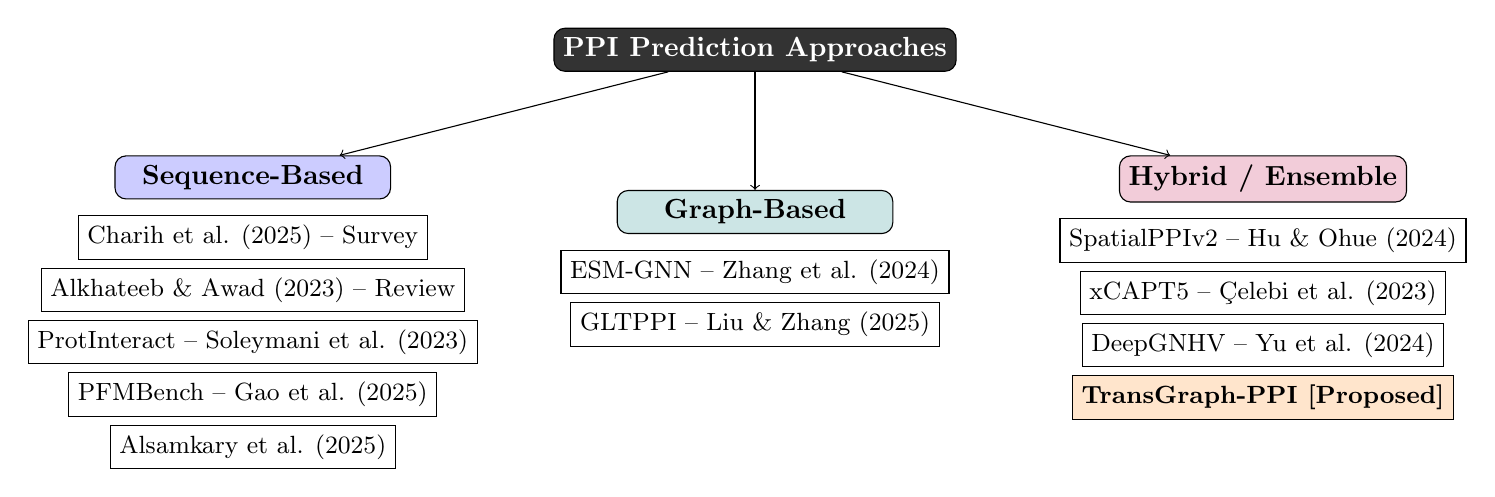
\begin{tikzpicture}[node distance=1.5cm, auto]
    % Nodes
    \node (top) [rectangle, draw, fill=black!80, text=white, minimum width=5cm, rounded corners] {\textbf{PPI Prediction Approaches}};
    
    \node (seq) [rectangle, draw, fill=blue!20, below left=of top, xshift=-1cm, minimum width=3.5cm, rounded corners] {\textbf{Sequence-Based}};
    \node (graph) [rectangle, draw, fill=teal!20, below=of top, minimum width=3.5cm, rounded corners] {\textbf{Graph-Based}};
    \node (hybrid) [rectangle, draw, fill=purple!20, below right=of top, xshift=1cm, minimum width=3.5cm, rounded corners] {\textbf{Hybrid / Ensemble}};
    
    % Sequence list
    \node (s1) [rectangle, draw, below=0.2cm of seq, font=\small, minimum width=3.5cm] {Charih et al. (2025) -- Survey};
    \node (s2) [rectangle, draw, below=0.1cm of s1, font=\small, minimum width=3.5cm] {Alkhateeb \& Awad (2023) -- Review};
    \node (s3) [rectangle, draw, below=0.1cm of s2, font=\small, minimum width=3.5cm] {ProtInteract -- Soleymani et al. (2023)};
    \node (s4) [rectangle, draw, below=0.1cm of s3, font=\small, minimum width=3.5cm] {PFMBench -- Gao et al. (2025)};
    \node (s5) [rectangle, draw, below=0.1cm of s4, font=\small, minimum width=3.5cm] {Alsamkary et al. (2025)};
    
    % Graph list
    \node (g1) [rectangle, draw, below=0.2cm of graph, font=\small, minimum width=3.5cm] {ESM-GNN -- Zhang et al. (2024)};
    \node (g2) [rectangle, draw, below=0.1cm of g1, font=\small, minimum width=3.5cm] {GLTPPI -- Liu \& Zhang (2025)};
    
    % Hybrid list
    \node (h1) [rectangle, draw, below=0.2cm of hybrid, font=\small, minimum width=3.5cm] {SpatialPPIv2 -- Hu \& Ohue (2024)};
    \node (h2) [rectangle, draw, below=0.1cm of h1, font=\small, minimum width=3.5cm] {xCAPT5 -- \c{C}elebi et al. (2023)};
    \node (h3) [rectangle, draw, below=0.1cm of h2, font=\small, minimum width=3.5cm] {DeepGNHV -- Yu et al. (2024)};
    \node (h4) [rectangle, draw, below=0.1cm of h3, font=\small, minimum width=3.5cm, fill=orange!20] {\textbf{TransGraph-PPI [Proposed]}};
    
    % Arrows
    \draw [->] (top) -- (seq);
    \draw [->] (top) -- (graph);
    \draw [->] (top) -- (hybrid);
\end{tikzpicture}
\caption{Taxonomy of PPI Prediction Methods: Sequence-Based, Graph-Based, and Hybrid Approaches}
\end{figure}

\newpage

% --- Page 26: Summary and Evolution Diagram ---
\section{Summary of Literature Survey}
The reviewed literature collectively establishes a clear trajectory in computational PPI prediction: from early traditional machine learning with handcrafted features, through CNN and RNN-based deep learning, to the current state-of-the-art that leverages transformer-based protein language models and graph neural networks.

Several key observations emerge from this survey:
\begin{enumerate}
    \item Protein language models (ESM-2, ProtT5, T5-XL) consistently outperform hand-crafted feature encodings by capturing rich evolutionary and biochemical information directly from amino acid sequences.
    \item Graph-based models (GCN, GAT, VGAE) excel at capturing topological and structural relationships that sequence-only models miss.
    \item Hybrid frameworks combining PLMs with GNNs achieve superior performance over either approach used in isolation.
    \item Ensemble methods and meta-learners (XGBoost, stacking) further improve robustness and generalization.
    \item Interpretability (SHAP, attention visualization) remains an underexplored but critical area for translating predictions into actionable drug discovery insights.
    \item Dataset quality, class imbalance, and cross-species generalization remain persistent challenges that the proposed TransGraph-PPI framework directly addresses.
\end{enumerate}

The proposed TransGraph-PPI framework synthesizes these insights by integrating ESM-2 embeddings with a GAT, using a stacking-based ensemble with XGBoost, and applying SHAP-based interpretability---representing a principled and comprehensive response to the limitations identified across the reviewed literature.

Figure 1.2 illustrates the chronological evolution of computational PPI prediction methods, culminating in the proposed TransGraph-PPI framework.

\begin{figure}[H]
\centering
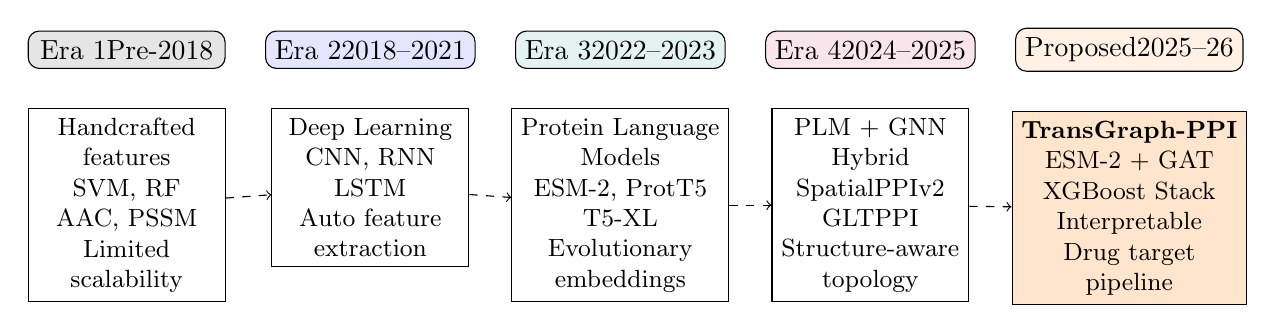
\begin{tikzpicture}[node distance=1cm, auto]
    % Eras
    \node (e1) [rectangle, draw, fill=gray!20, minimum width=2.5cm, rounded corners] {Era 1 \\ Pre-2018};
    \node (e2) [rectangle, draw, fill=blue!10, right=0.5cm of e1, minimum width=2.5cm, rounded corners] {Era 2 \\ 2018--2021};
    \node (e3) [rectangle, draw, fill=teal!10, right=0.5cm of e2, minimum width=2.5cm, rounded corners] {Era 3 \\ 2022--2023};
    \node (e4) [rectangle, draw, fill=purple!10, right=0.5cm of e3, minimum width=2.5cm, rounded corners] {Era 4 \\ 2024--2025};
    \node (e5) [rectangle, draw, fill=orange!10, right=0.5cm of e4, minimum width=2.5cm, rounded corners] {Proposed \\ 2025--26};
    
    % Details
    \node (d1) [rectangle, draw, below=0.5cm of e1, font=\small, minimum width=2.5cm, align=center] {Handcrafted \\ features \\ SVM, RF \\ AAC, PSSM \\ Limited \\ scalability};
    \node (d2) [rectangle, draw, below=0.5cm of e2, font=\small, minimum width=2.5cm, align=center] {Deep Learning \\ CNN, RNN \\ LSTM \\ Auto feature \\ extraction};
    \node (d3) [rectangle, draw, below=0.5cm of e3, font=\small, minimum width=2.5cm, align=center] {Protein Language \\ Models \\ ESM-2, ProtT5 \\ T5-XL \\ Evolutionary \\ embeddings};
    \node (d4) [rectangle, draw, below=0.5cm of e4, font=\small, minimum width=2.5cm, align=center] {PLM + GNN \\ Hybrid \\ SpatialPPIv2 \\ GLTPPI \\ Structure-aware \\ topology};
    \node (d5) [rectangle, draw, below=0.5cm of e5, font=\small, minimum width=2.5cm, align=center, fill=orange!20] {\textbf{TransGraph-PPI} \\ ESM-2 + GAT \\ XGBoost Stack \\ Interpretable \\ Drug target \\ pipeline};
    
    % Arrows
    \draw [->, dashed] (d1) -- (d2);
    \draw [->, dashed] (d2) -- (d3);
    \draw [->, dashed] (d3) -- (d4);
    \draw [->, dashed] (d4) -- (d5);
\end{tikzpicture}
\caption{Evolution of Computational PPI Prediction Methods from Traditional ML to TransGraph-PPI}
\end{figure}

\newpage

% --- Page 27: Research Gap Analysis ---
\section{Research Gap Analysis: Existing Limitations and Proposed Solution}
Figure 1.3 maps the key limitations identified across the surveyed literature against the specific solutions offered by the proposed TransGraph-PPI framework.

\begin{figure}[H]
\centering
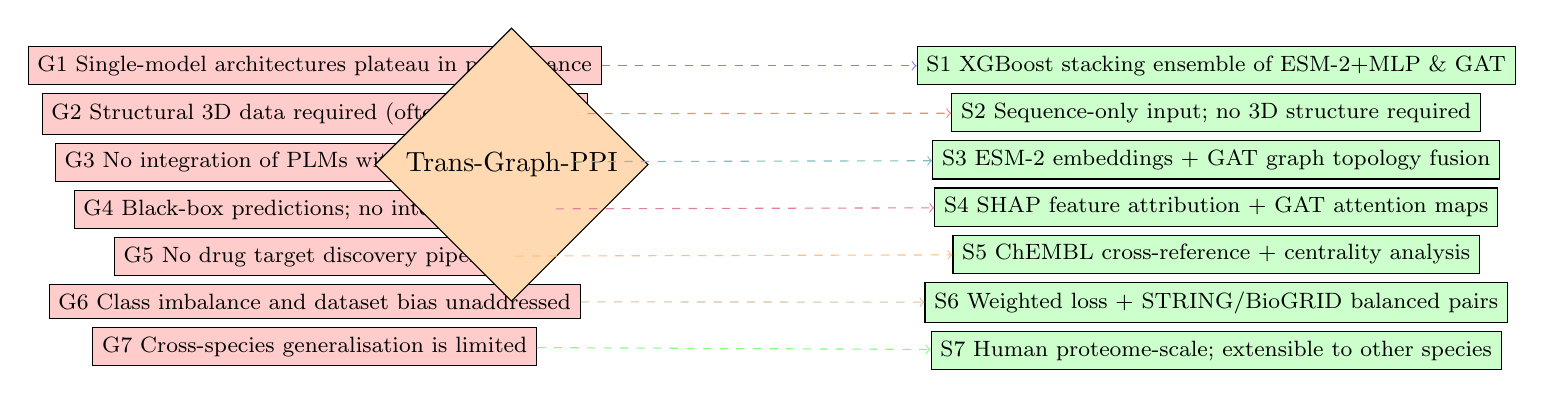
\begin{tikzpicture}[node distance=1cm, auto]
    % Problems list
    \node (p1) [rectangle, draw, fill=red!20, font=\footnotesize, minimum width=5cm, align=left] {G1 Single-model architectures plateau in performance};
    \node (p2) [rectangle, draw, fill=red!20, below=0.1cm of p1, font=\footnotesize, minimum width=5cm, align=left] {G2 Structural 3D data required (often unavailable)};
    \node (p3) [rectangle, draw, fill=red!20, below=0.1cm of p2, font=\footnotesize, minimum width=5cm, align=left] {G3 No integration of PLMs with graph topology};
    \node (p4) [rectangle, draw, fill=red!20, below=0.1cm of p3, font=\footnotesize, minimum width=5cm, align=left] {G4 Black-box predictions; no interpretability};
    \node (p5) [rectangle, draw, fill=red!20, below=0.1cm of p4, font=\footnotesize, minimum width=5cm, align=left] {G5 No drug target discovery pipeline};
    \node (p6) [rectangle, draw, fill=red!20, below=0.1cm of p5, font=\footnotesize, minimum width=5cm, align=left] {G6 Class imbalance and dataset bias unaddressed};
    \node (p7) [rectangle, draw, fill=red!20, below=0.1cm of p6, font=\footnotesize, minimum width=5cm, align=left] {G7 Cross-species generalisation is limited};

    % Solutions list
    \node (s1) [rectangle, draw, fill=green!20, right=4cm of p1, font=\footnotesize, minimum width=5cm, align=left] {S1 XGBoost stacking ensemble of ESM-2+MLP \& GAT};
    \node (s2) [rectangle, draw, fill=green!20, below=0.1cm of s1, font=\footnotesize, minimum width=5cm, align=left] {S2 Sequence-only input; no 3D structure required};
    \node (s3) [rectangle, draw, fill=green!20, below=0.1cm of s2, font=\footnotesize, minimum width=5cm, align=left] {S3 ESM-2 embeddings + GAT graph topology fusion};
    \node (s4) [rectangle, draw, fill=green!20, below=0.1cm of s3, font=\footnotesize, minimum width=5cm, align=left] {S4 SHAP feature attribution + GAT attention maps};
    \node (s5) [rectangle, draw, fill=green!20, below=0.1cm of s4, font=\footnotesize, minimum width=5cm, align=left] {S5 ChEMBL cross-reference + centrality analysis};
    \node (s6) [rectangle, draw, fill=green!20, below=0.1cm of s5, font=\footnotesize, minimum width=5cm, align=left] {S6 Weighted loss + STRING/BioGRID balanced pairs};
    \node (s7) [rectangle, draw, fill=green!20, below=0.1cm of s6, font=\footnotesize, minimum width=5cm, align=left] {S7 Human proteome-scale; extensible to other species};

    % Center node
    \node (center) [diamond, draw, fill=orange!30, midway, xshift=2.5cm, yshift=-3cm] {Trans-Graph-PPI};

    % Links
    \draw [->, dashed, blue!50] (p1) -- (s1);
    \draw [->, dashed, red!50] (p2) -- (s2);
    \draw [->, dashed, teal!50] (p3) -- (s3);
    \draw [->, dashed, purple!50] (p4) -- (s4);
    \draw [->, dashed, orange!50] (p5) -- (s5);
    \draw [->, dashed, brown!50] (p6) -- (s6);
    \draw [->, dashed, green!50] (p7) -- (s7);
\end{tikzpicture}
\caption{Research Gap Analysis: Existing Literature Limitations vs. TransGraph-PPI Solutions}
\end{figure}

\newpage

% --- Page 28: Critical Analysis ---
\section{Critical Analysis: Importance, Novelty, and Contribution of TransGraph-PPI}
\subsection{Why Is the Chosen Problem Important?}
Protein–Protein Interactions (PPIs) are the molecular machinery underlying virtually every biological process—from immune response and signal transduction to cell cycle regulation and disease progression. Dysregulation of PPIs is directly implicated in cancer, neurodegenerative disorders, infectious diseases, and autoimmune conditions, making the identification of interacting protein pairs not merely an academic exercise but a fundamental prerequisite for therapeutic intervention. Despite decades of experimental effort, the experimentally confirmed PPI network covers only a small fraction of the estimated hundreds of thousands of interactions in the human proteome. Traditional experimental methods such as yeast two-hybrid screening, co-immunoprecipitation, and affinity purification mass spectrometry are costly, slow, prone to high false-positive rates, and fundamentally unsuited to the scale of modern proteomics. The rapid expansion of protein sequence databases—UniProt now contains over 250 million sequences—has created an urgent and unmet need for computational methods that can predict interactions accurately, at scale, and from sequence data alone. Computational PPI prediction therefore sits at the intersection of bioinformatics, machine learning, and drug discovery, with direct and measurable impact on how candidate therapeutic targets are identified and validated.

\subsection{What Is Novel in the Proposed Contribution?}
The proposed TransGraph-PPI framework introduces a principled integration of three complementary computational paradigms—protein language model embeddings, graph attention-based topology learning, and ensemble meta-learning—into a single end-to-end PPI prediction system, augmented by biologically grounded analytical modules. The novelty comprises five key dimensions: (1) ESM-2 embeddings replace all handcrafted features and require no 3D structural data; (2) a GAT simultaneously models protein interaction network topology; (3) a stacking ensemble with XGBoost combines the complementary base model outputs in a learnable, data-driven way; (4) SHAP-based interpretability and GAT attention visualization provide residue-level and feature-level explanations; (5) the framework extends beyond binary PPI prediction to include mutation impact scanning, subcellular localization filtering, network centrality analysis, and ChEMBL drug target prioritization.

\subsection{How Does TransGraph-PPI Advance the State-of-the-Art?}
TransGraph-PPI advances the state-of-the-art by simultaneously closing the key gaps identified across the literature: structural data dependency (eliminated), single-model representational limits (overcome by the ensemble), absence of interpretability (addressed by SHAP), and lack of a drug discovery pipeline (addressed via ChEMBL and centrality analysis). By combining ESM-2 with GAT in a stacking ensemble, the system is positioned to outperform the best sequence-only models (xCAPT5, ProtInteract) and graph-only models (GNN-PPI, GLTPPI), while being more broadly applicable than structure-dependent methods (SpatialPPIv2, DeepGNHV).

\newpage

% --- Page 29: Critical Analysis (Continued) ---
\subsection{How Does TransGraph-PPI Differ from Each Surveyed Work?}
Compared to Charih et al. [1], TransGraph-PPI implements a concrete validated architecture rather than a survey. Relative to Alkhateeb and Awad [2], TransGraph-PPI realizes the GCN + ensemble vision using ESM-2 and XGBoost. SpatialPPIv2 [3] depends on 3D structures; TransGraph-PPI does not. ProtInteract [4] uses physicochemical features and no graph modeling; TransGraph-PPI replaces both. xCAPT5 [5] applies XGBoost as a flat single-model classifier; TransGraph-PPI uses it as a stacking meta-learner integrating two heterogeneous base models. DeepGNHV [6] is limited to human–virus interactions and requires AlphaFold. The hierarchical pooling work [7] targets affinity prediction with no interaction network or drug analysis. ESM-GNN [8] predicts interaction sites on individual proteins, not pairwise binary PPI. PFMBench [9] is a benchmark framework, not a predictor. GLTPPI [10], the most architecturally similar, lacks an ensemble, interpretability, mutation analysis, and drug target pipeline—all integral to TransGraph-PPI.

\newpage

% --- Page 30: Bibliography ---
\chapter*{Bibliography}
\addcontentsline{toc}{chapter}{Bibliography}

\begin{enumerate}
    \item[[1]] F. Charih, J. R. Green, and K. K. Biggar, ``Sequence-Based Protein–Protein Interaction Prediction and Its Applications in Drug Discovery,'' \textit{Cells}, vol. 14, no. 18, p. 1449, Sep. 2025.
    \item[[2]] N. Alkhateeb and M. Awad, ``Advances in Protein–Protein Interaction Prediction: A Deep Learning Perspective,'' \textit{Bioinformatics Journal Review}, 2023.
    \item[[3]] W. Hu and M. Ohue, ``SpatialPPIv2: Enhancing Protein–Protein Interaction Prediction through Graph Neural Networks with Protein Language Models,'' \textit{Bioinformatics Advances}, 2024.
    \item[[4]] F. Soleymani, E. Paquet, H. L. Viktor, W. Michalowski, and D. Spinello, ``ProtInteract: A Deep Learning Framework for Predicting Protein–Protein Interactions,'' \textit{Computational Biology and Medicine}, 2023.
    \item[[5]] M. \c{C}elebi et al., ``xCAPT5: Protein–Protein Interaction Prediction Using Protein Language Model Embeddings and Deep Learning,'' \textit{Bioinformatics}, 2023.
    \item[[6]] Z. Yu et al., ``Graph Neural Network Integrated with Pretrained Protein Language Model for Predicting Human–Virus Protein–Protein Interactions,'' \textit{Bioinformatics}, 2024.
    \item[[7]] M. Alsamkary et al., ``Beyond Simple Concatenation: Fairly Assessing PLM Architectures for Multi-Chain Protein-Protein Interaction Prediction,'' \textit{Bioinformatics Advances}, 2025.
    \item[[8]] J. Zhang et al., ``Predicting Human Protein-Protein Interaction Sites by Integrating ESM-2 Sequence Embeddings and a Gated Graph Neural Network,'' \textit{Bioinformatics}, 2024.
    \item[[9]] Z. Gao et al., ``PFMBench – Protein Foundation Model Benchmark,'' \textit{Nature Methods} (preprint), 2025.
    \item[[10]] J. Liu and T. Zhang, ``ESM2-Driven Protein-Protein Interaction Prediction with Global-Local Graph Topology Learning,'' \textit{Briefings in Bioinformatics}, 2025.
\end{enumerate}

\end{document}
